\chapter{Introduction}

\section{Overview}
\label{Intro: Overiew}

\section{Research context}
\label{Intro: ResearchContext}

\section{Research aim and questions}
\label{Intro:RQ}
The research described in this thesis explores the following research aim:
\begin{quote}
    \textit{``How might participation be configured for people with dementia to shape the design process of technology''}
\end{quote}
This research aim is split into three research questions, to provide insights into the experiences and perspectives of stakeholders commonly implicated in design processes in designing with and for people with dementia, intending to broaden the conversation surrounding technology design with and for people with dementia. The following section introduces each research question followed by a description.

\subsection{Research question one}
\label{RQ1}
\begin{quote}
\textit{``How can we use participatory design approaches to provide meaningful and engaging experiences for people with dementia?''}
\end{quote}
In exploring this question, the methodologies used in this thesis explore the ways to move toward more inclusive design approaches that require flexible configuration to support the different needs of participants. Further, this exploration draws attention to how we talk about dementia, to what extent people with dementia want to contribute to technology design, and ways to ensure the person with dementia is respected and engaged in research.

\subsection{Research question two}
\label{RQ2}
\begin{quote}
\textit{``What are the ethical implications for people with dementia to participate in HCI research?''}
\end{quote}
Given that people with dementia may experience changes to their ability to problem solve, increasing need for care, and make judgements, many of the social and cognitive consequences of living with dementia can be seen as ethical challenges, making it a complex space for research. With this in mind, the thesis examines ethical practices used in dementia-HCI research to present insights into the careful ethical considerations required when working with people with dementia and their families. 

\subsection{Research question three}
\label{RQ3}
\begin{quote}
\textit{``What are the competing interests and expectations to support meaningful dialogue in dementia design research when involving multiple stakeholders - such as people with dementia, developers, designers and researchers?''}
\end{quote}
For the final research question, the thesis investigates the importance of designing for multiple interests and workflows to ensure that stakeholders who are part of the design process to support collaboration and engagement between the diverse stakeholders. 

\section{Thesis structure}
\label{Intro: Thesis structure}
In this section, I describe the structure of the thesis:

\subsection{Chapter two - Background Literature}
\label{Intro:ChapterTwo}
This chapter aims to describe prior work discussing how people with dementia have been represented and involved in technology design and development. Initially, this chapter reviews the involvement of people with dementia in dementia-HCI work that draws attention to a strong relational basis for design practice. Following the review of dementia-HCI work, I highlight three areas that require investigation. From here, I draw from outside the HCI literature that examines the type of ethical dilemmas; public perception of dementia, and involving later stages of dementia in the co-creation process. Finally, to conclude this chapter, I describe four areas of interest to this thesis that might broaden our understanding of how to design and develop technology for and with people with dementia.

\subsection{Chapter three - Methodology}
\label{Intro:ChapterThree}
In the methodology chapter, I explain and justify the research approach taken in the thesis that shapes the data chapters. First, I introduce the epistemological approach adopted in this thesis. Following, I describe how I adapt co-design and participatory design to fit the needs of people with dementia. I then unpack participatory methods in dementia and HCI that emphasise the need to adopt approaches to fit the needs of people with dementia. I discuss the ethical complexities of the thesis; the data collection of the four data chapters; overview of recruitment and location; and the qualitative data analysis method, thematic analysis and reflexive practice. Moreover, I detail the analytical and reliability approaches I undertake in this thesis to provide work that is more mindful of the assumptions and methodological choices made within this thesis.

\subsection{Chapter four - Sharing a Virtual World with People with Dementia: A Reflective Account}
\label{Intro:ChapterFour}
The chapter is a reflective account highlighting several themes and reasons for the subsequent chapters. This chapter reflects on two studies working with people with dementia and their families to design virtual reality experiences. Both studies worked closely with a dementia café in Newcastle called Silverline Memories, which provide activities and organise celebrations for members' birthdays and other special occasions. By working closely with families with dementia, the account examines how I adapted participatory approaches to involve people with dementia in more sensitive and meaningful ways. Further, by working with family members as well as the person with dementia, I recognise that many of the challenges in designing technology with people with dementia should consider the needs and interests of the ecology of care. In that respect, this chapter takes a reflective approach to provide a clear account of my background, history, the perspective on dementia, and design approaches that ultimately impact the participants, the setting and the overarching work. As such, this chapter provides insights into designing VR environments for families with dementia and a personal narrative, that recognises the concerns, dilemmas, and the impact of working within sensitive research spaces.

\subsection{Chapter five - DemVR: Exploring Shifting Sensitivities in a Hackathon for Dementia}
\label{Intro:ChapterFive}
Following the two studies focusing on the inclusive design of virtual reality experiences for families living with dementia, I was curious about how designing bespoke and sensitive VR experiences might function in larger-scale community events. As I described in chapter four, learning to design within such a complex topic required extensive time working with people with dementia. However, developers and designers who work on bringing dementia technology to the market, will unlikely have the chance to work with people with dementia to the extent I could. As such, this chapter explores the design of a hackathon, DemVR, both to generate a set of bespoke VR environments for those with dementia and consider how developers/designers and people with dementia may collaborate.

The event consists of two stages: a six-week engagement phase to support participants in proposing and refining initial ideas online; and a two-day hackathon inviting designers and domain experts to develop their ideas further. While the event gained reasonable interest from designers, developers, and students throughout both phases, the representation of people with dementia and their care partners was limited. The chapter examines the structure of the event and the role this played in the struggle to involve people with dementia and their care partners. The data analysis presents insights into participants’ motivations, design approaches to accommodate the absent user, and the design ideas that the teams developed to address the social context of the user. Against a background of the extant literature on reification in design, collaborative design events, and dementia, the discussion provides a series of commitments for HCI and dementia research. The commitments offer insights into how we might mitigate stereotypes in constructing the end-user; ways to improve recruitment for involving marginalised populations in events; and steps to promote more inclusive, community-driven events. 

\subsection{Chapter six - Learning from Ethics in Dementia Research}
\label{Intro:ChapterSix}

\subsection{Chapter seven - Co-creating a Digital Toolkit to Support Design for Dementia}
\label{Intro:ChapterSeven}
From the data analysed in the previous chapters, it was apparent that a) representing people with dementia can be difficult in public events and causes multiple knock-on effects on design outputs; and b) future research work in dementia should aim to be participant-led and shift towards creating tools or processes to promote conversations between people with dementia and stakeholders commonly implicated in design processes.

In response, this chapter presents the design of the Dialogical Dementia Design (D3) toolkit, a set of resources to support co-designing with people with dementia. The study invited designers and developers and people with dementia to participate in interactive workshops and interviews that explored resources needed by developers and designers to design with people with dementia and investigate how people with dementia envision their potential participation with toolkits. Through iterative engagement with participant data, I surfaced a set of design priorities that helped shape a prototype of the toolkit. This toolkit comprised several components that offered opportunities to learn and engage in sensitive ways with people with dementia. Analysis of participant reactions to the designed prototype raises questions around the challenges of co-creation through safety and privacy, the sharing of the ‘designer’ role between the different stakeholders, and finally, the type of incentives required for participation and engagement in curating a toolkit. Against a background of extant literature on dementia and collaboration, the discussion provides a series of directions for HCI and dementia research, highlighting how we might balance participants' privacy, safety, and due recognition; priorities in growing a community-owned toolkit; and the accountability and responsibility that designers and developers carry in adapting their working practices for designing within sensitive areas.
\subsection{Chapter eight - Discussion and Future Work}
\label{Intro:ChapterEight}


\subsection{Thesis map}
For chapters four to seven, I present a map of which represents the different research questions each data chapter tackles (see figure \ref{fig:RQ_and_Chapters}).

\label{Intro:Thesis Map}
\begin{figure}[htp]
\centering
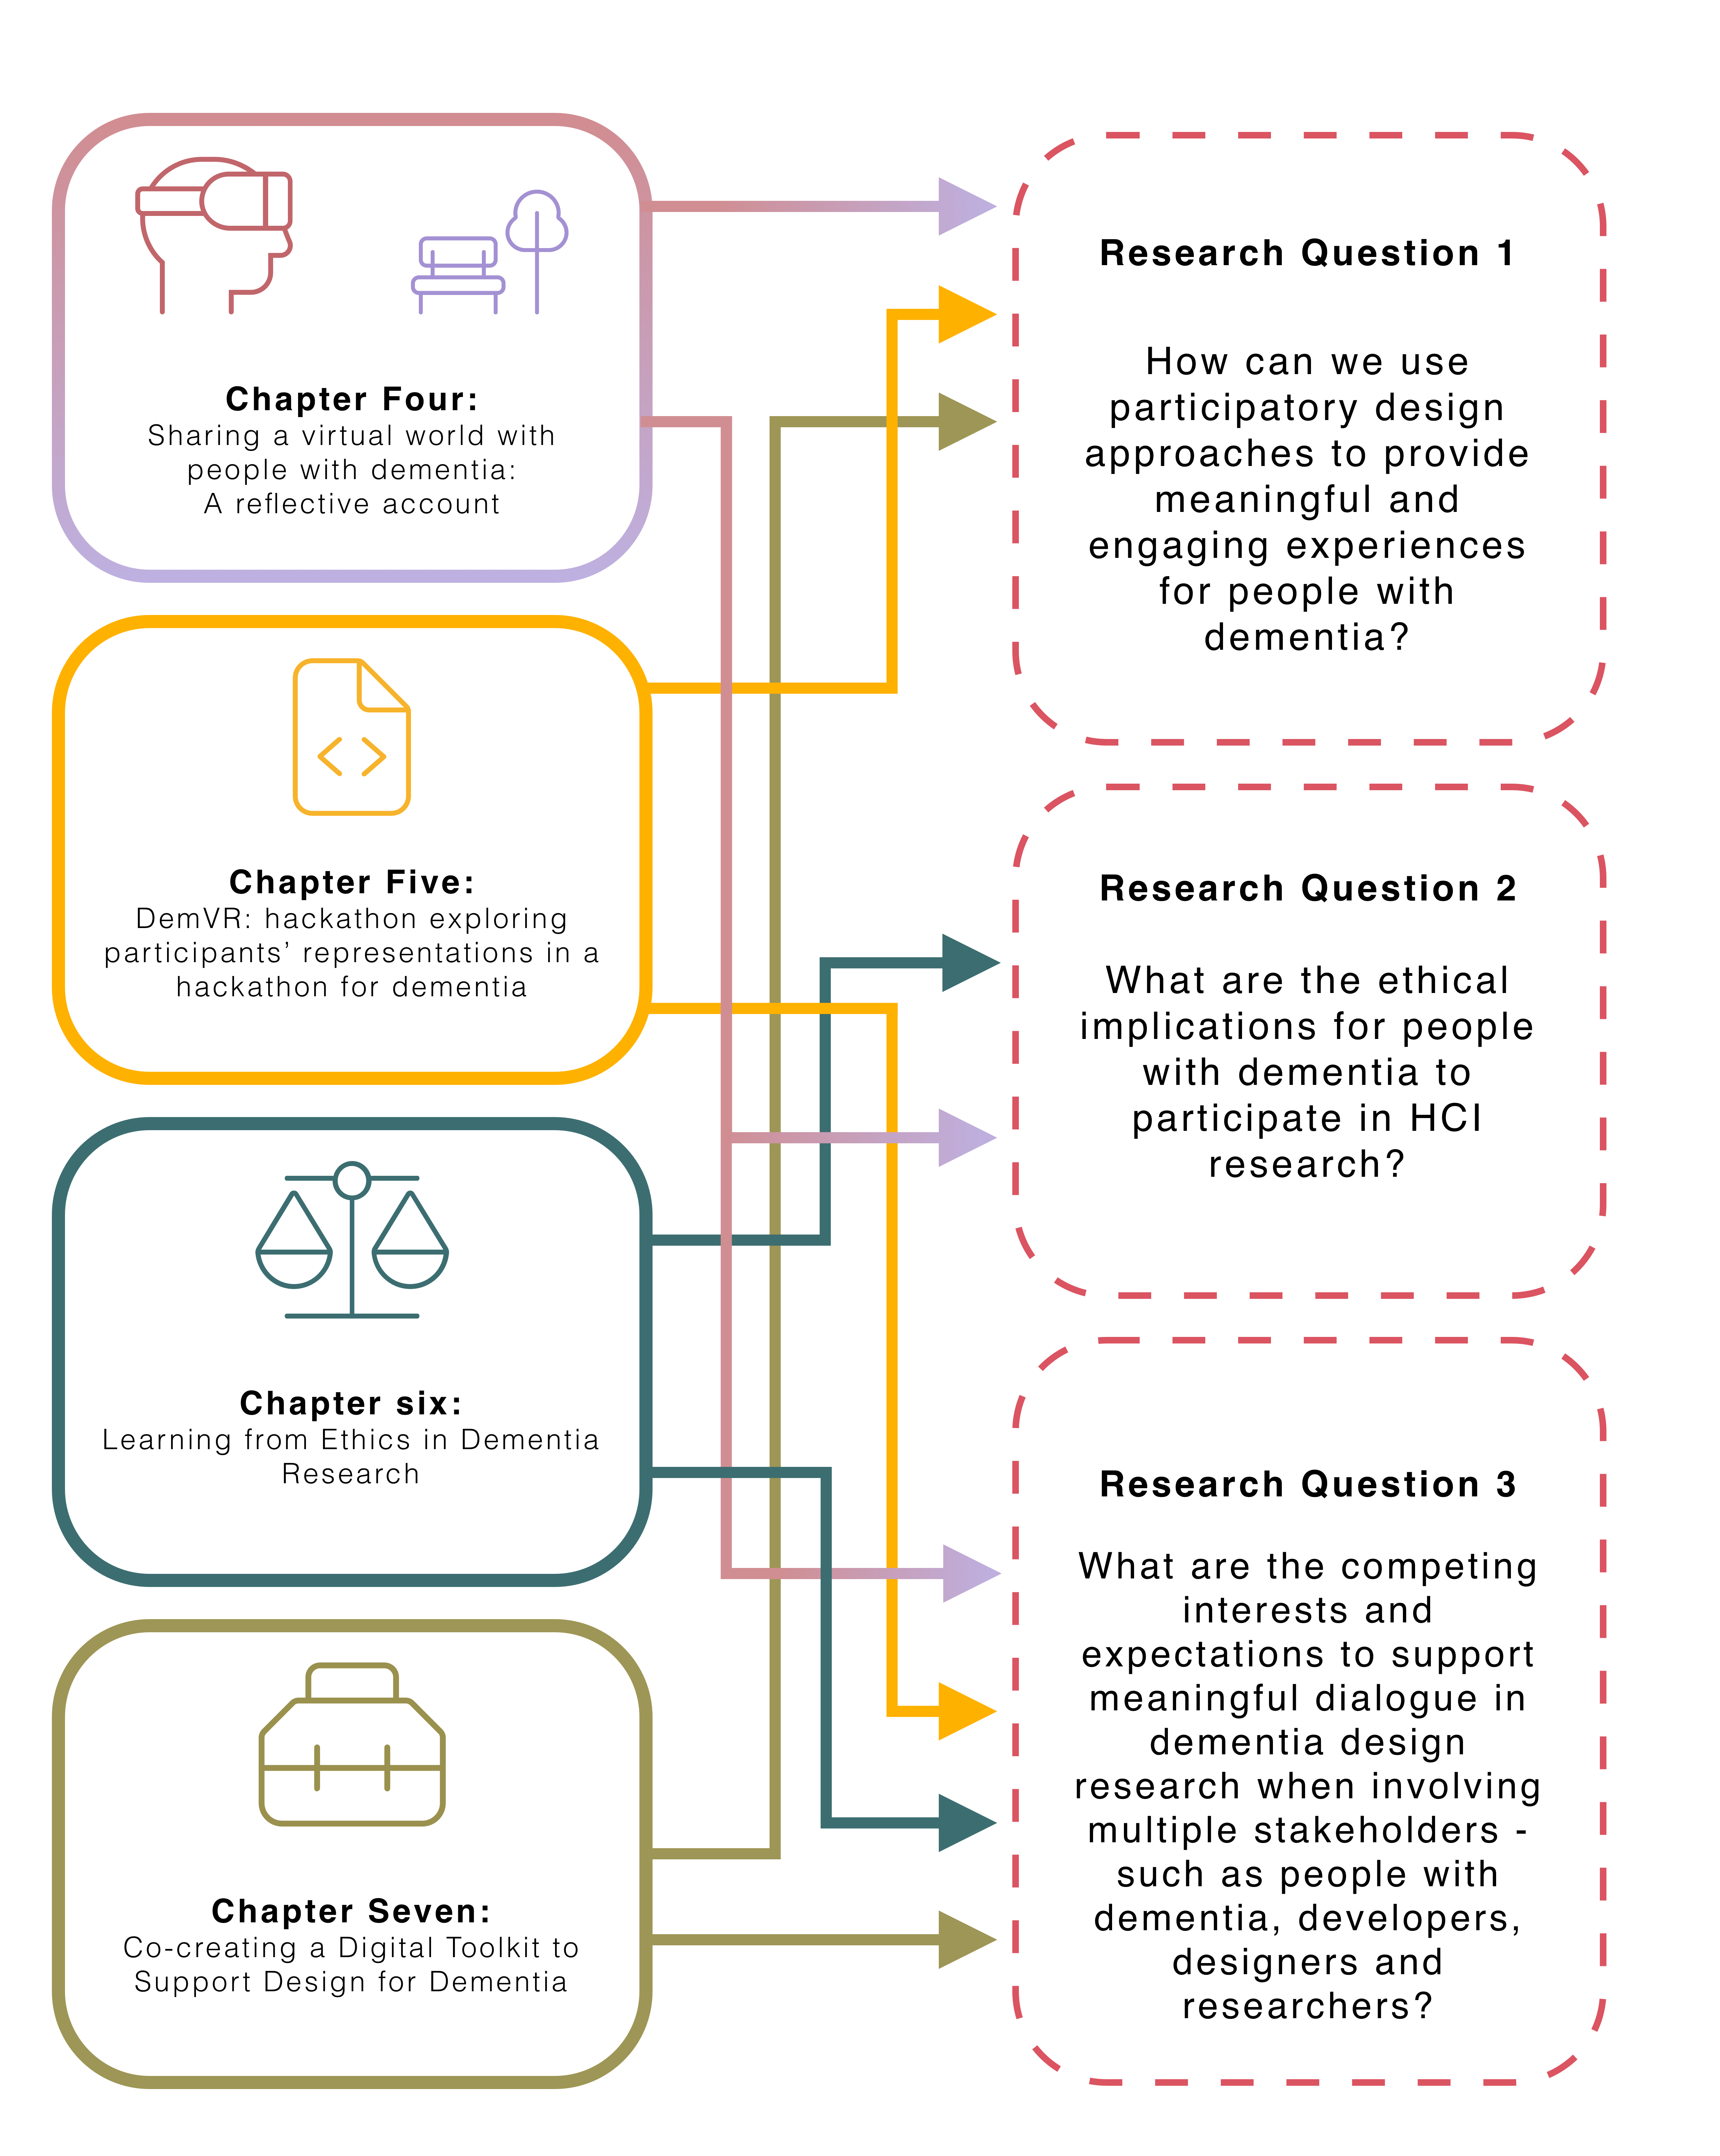
\includegraphics[width=.8\linewidth]{Images/Thesis_Narrative/RQ_and_Chapters.png}
\caption{Thesis Map showing the relationships between data chapters to research questions}
\label{fig:RQ_and_Chapters}
\end{figure}


\section{Contributions}
\label{Intro:Contribution}

\section{Summary}
\label{Intro: Summary}